
%----------------------------------------------------------------------------------
\begin{frame}[fragile]{Code Generation Phase}{}
%----------------------------------------------------------------------------------

\begin{figure}
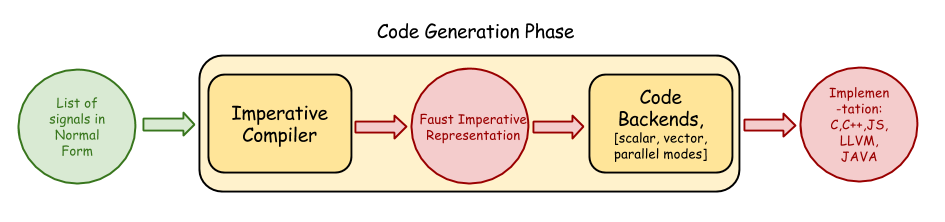
\includegraphics[width=1\columnwidth]{images/code-generation-chain}
\end{figure}

\end{frame}


%----------------------------------------------------------------------------------
\begin{frame}[fragile]{Code Generation Phase}{Four Code generation modes}
%----------------------------------------------------------------------------------

\begin{figure}
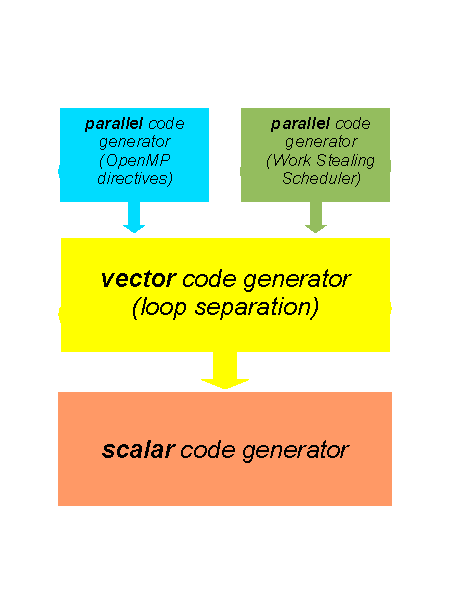
\includegraphics[width=0.5\columnwidth]{images/compiler-stack1}
\end{figure}

\end{frame}
 

 
%----------------------------------------------------------------------------------
\begin{frame}[fragile]{Code Generation Phase}{two 1-pole filters in parallel connected to an adder}
%----------------------------------------------------------------------------------
\begin{lstlisting}[basicstyle=\ttfamily\tiny\color{yotxt}]

   filter(c) = *(1-c) : + ~ *(c);
   process = filter(0.9), filter(0.9) : +;
   
\end{lstlisting}
   
\begin{center}
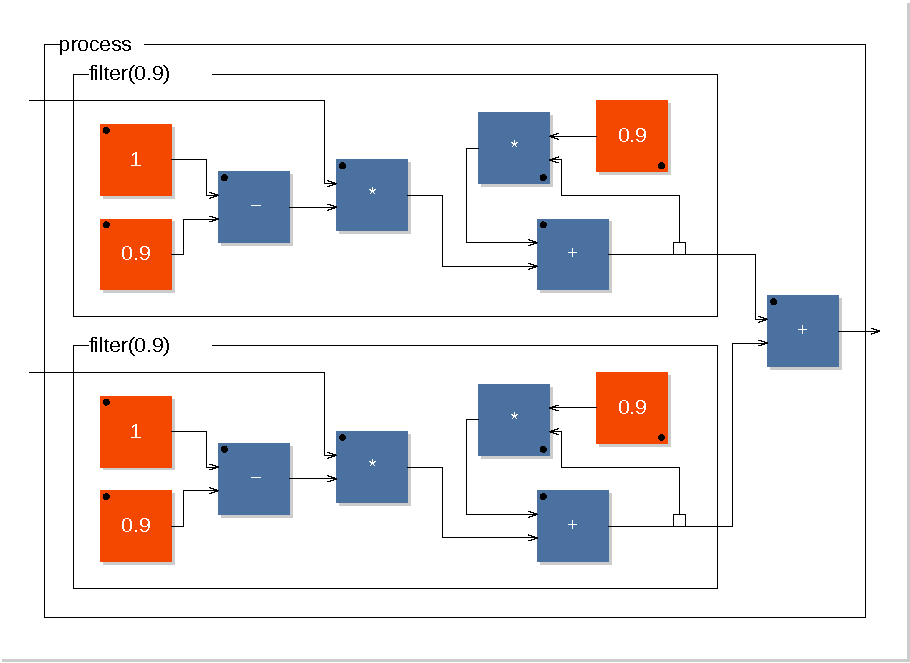
\includegraphics[width=7cm]{images/filter2.pdf}
\end{center}
\end{frame}
 

 
 %----------------------------------------------------------------------------------
\begin{frame}[fragile]{Code Generation Phase}{Scalar Code}
 %----------------------------------------------------------------------------------
\begin{lstlisting}[basicstyle=\ttfamily\tiny\color{yotxt}]

   virtual void compute (int count, float** input, float** output) {
     float* input0 = input[0];
     float* input1 = input[1];
     float* output0 = output[0];
     for (int i=0; i<count; i++) {
       fRec0[0] = (0.1f * input1[i]) + (0.9f * fRec0[1]);
       fRec1[0] = (0.1f * input0[i]) + (0.9f * fRec1[1]);
       output0[i] = (fRec1[0] + fRec0[0]);
       // post processing
       fRec1[1] = fRec1[0];
       fRec0[1] = fRec0[0];
     }
   }
   
\end{lstlisting}
\end{frame}
 
 %%%fRec1[0] = ((0.2f * (float)input0[i]) + (0.8f * fRec1[1]));
 			


 
 %----------------------------------------------------------------------------------
\begin{frame}{Code Generation Phase}{Vector Code}
 %----------------------------------------------------------------------------------
\framesubtitle{Loop Separation}
The \textit{Vector} Compilation Backend simplifies the autovectorization work of the C++ compiler by splitting the sample processing loop into several simpler loops. 

   \begin{figure}[h]
     \centering
 	\parbox{.4\linewidth}{
 		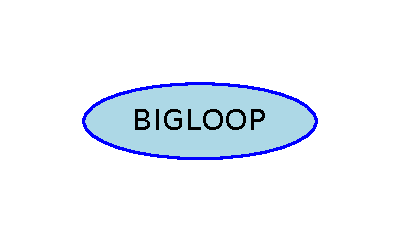
\includegraphics[scale=0.8]{images/singleloop}
 	}
   $\Rightarrow$ 
 	\parbox{.4\linewidth}{
 		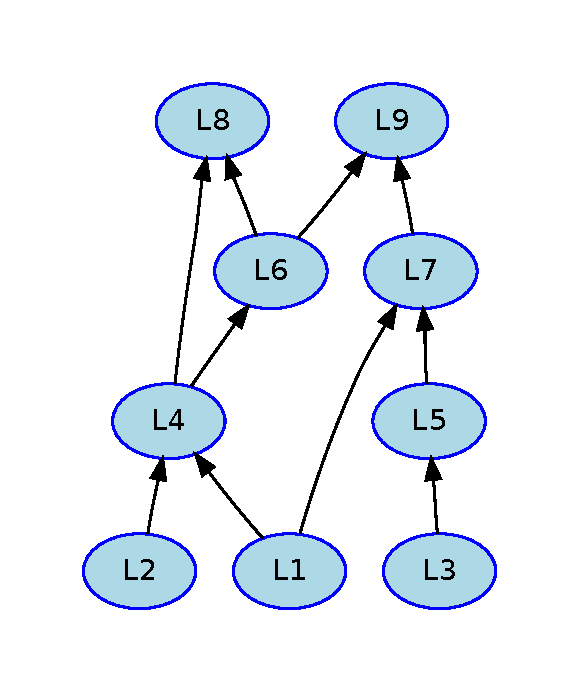
\includegraphics[scale=0.5]{images/loopgraph2}
 	}
   \end{figure}  
\end{frame}
 
 
 
 
 %----------------------------------------------------------------------------------
\begin{frame}[fragile]{Code Generation Phase}{Vector Code}
 %----------------------------------------------------------------------------------
\begin{lstlisting}[basicstyle=\ttfamily\tiny\color{yotxt}]
   ...
   // SECTION : 1
   for (int i=0; i<count; i++) {
     fRec0[i] = (0.1f * input1[i]) + (0.9f * fRec0[i-1]);
   }
   for (int i=0; i<count; i++) {
     fRec1[i] = (0.1f * input0[i]) + (0.9f * fRec1[i-1]);
   }
   // SECTION : 2
   for (int i=0; i<count; i++) {
     output0[i] = fRec1[i] + fRec0[i];
   }
   ...
\end{lstlisting}
\end{frame}
 
 

 
%----------------------------------------------------------------------------------
\begin{frame}[fragile]{Code Generation Phase}{Parallel Code -- OpenMP}
%----------------------------------------------------------------------------------
\begin{lstlisting}[basicstyle=\ttfamily\tiny\color{yotxt}]
 ...
 // SECTION : 1
 #pragma omp sections 
 { 
   #pragma omp section 
   for (int i=0; i<count; i++) {
     fRec0[i] = (0.1f * input1[i]) + (0.9f * fRec0[i-1]);
   }
   #pragma omp section 
   for (int i=0; i<count; i++) {
     fRec1[i] = (0.1f * input0[i]) + (0.9f * fRec1[i-1]);
   }
 } 
 // SECTION : 2
 #pragma omp for 
 for (int i=0; i<count; i++) {
   output0[i] = (fRec1[i] + fRec0[i]);
 }
 ...
\end{lstlisting}
\end{frame}

%----------------------------------------------------------------------------------
\begin{frame}[fragile]{Code Generation Phase}{Parallel Code -- Work Stealing}
%----------------------------------------------------------------------------------
\begin{lstlisting}[basicstyle=\ttfamily\tiny\color{yotxt}]

taskqueue.InitTaskList(task_list_size, task_list, fDynamicNumThreads, 
                                                  cur_thread, tasknum);
while (!fIsFinished) {
  switch (tasknum) {
    case WORK_STEALING_INDEX: { 
      tasknum = TaskQueue::GetNextTask(cur_thread, fDynamicNumThreads);
      break;
    }case LAST_TASK_INDEX: { 
      fIsFinished = true;
      break;
    }case 2: { 
      // LOOP 0x7fd873509e00
      ....
      fGraph.ActivateOneOutputTask(taskqueue,4,tasknum);
      break;
    }case 3: { 
      // LOOP 0x7fd873703d70
      ....				
      fGraph.ActivateOneOutputTask(taskqueue,4,tasknum);
      break;
    }case 4: { 
      // LOOP 0x7fd873509d20
      ....
      tasknum = LAST_TASK_INDEX;
      break;
    } 
  }
};
\end{lstlisting}
\end{frame}

\begin{frame}[fragile]{Code Generation Phase}{What improvements to expect from parallelized code ?}
\begin{block}{Sonik Cube}
Audio-visual installation involving a cube of light, reacting to sounds, immersed in an audio feedback room (Trafik/Orlarey 2006). 
\end{block}

\begin{columns}

 \begin{column}{0.55\textwidth}
	\begin{figure}
	\centering
	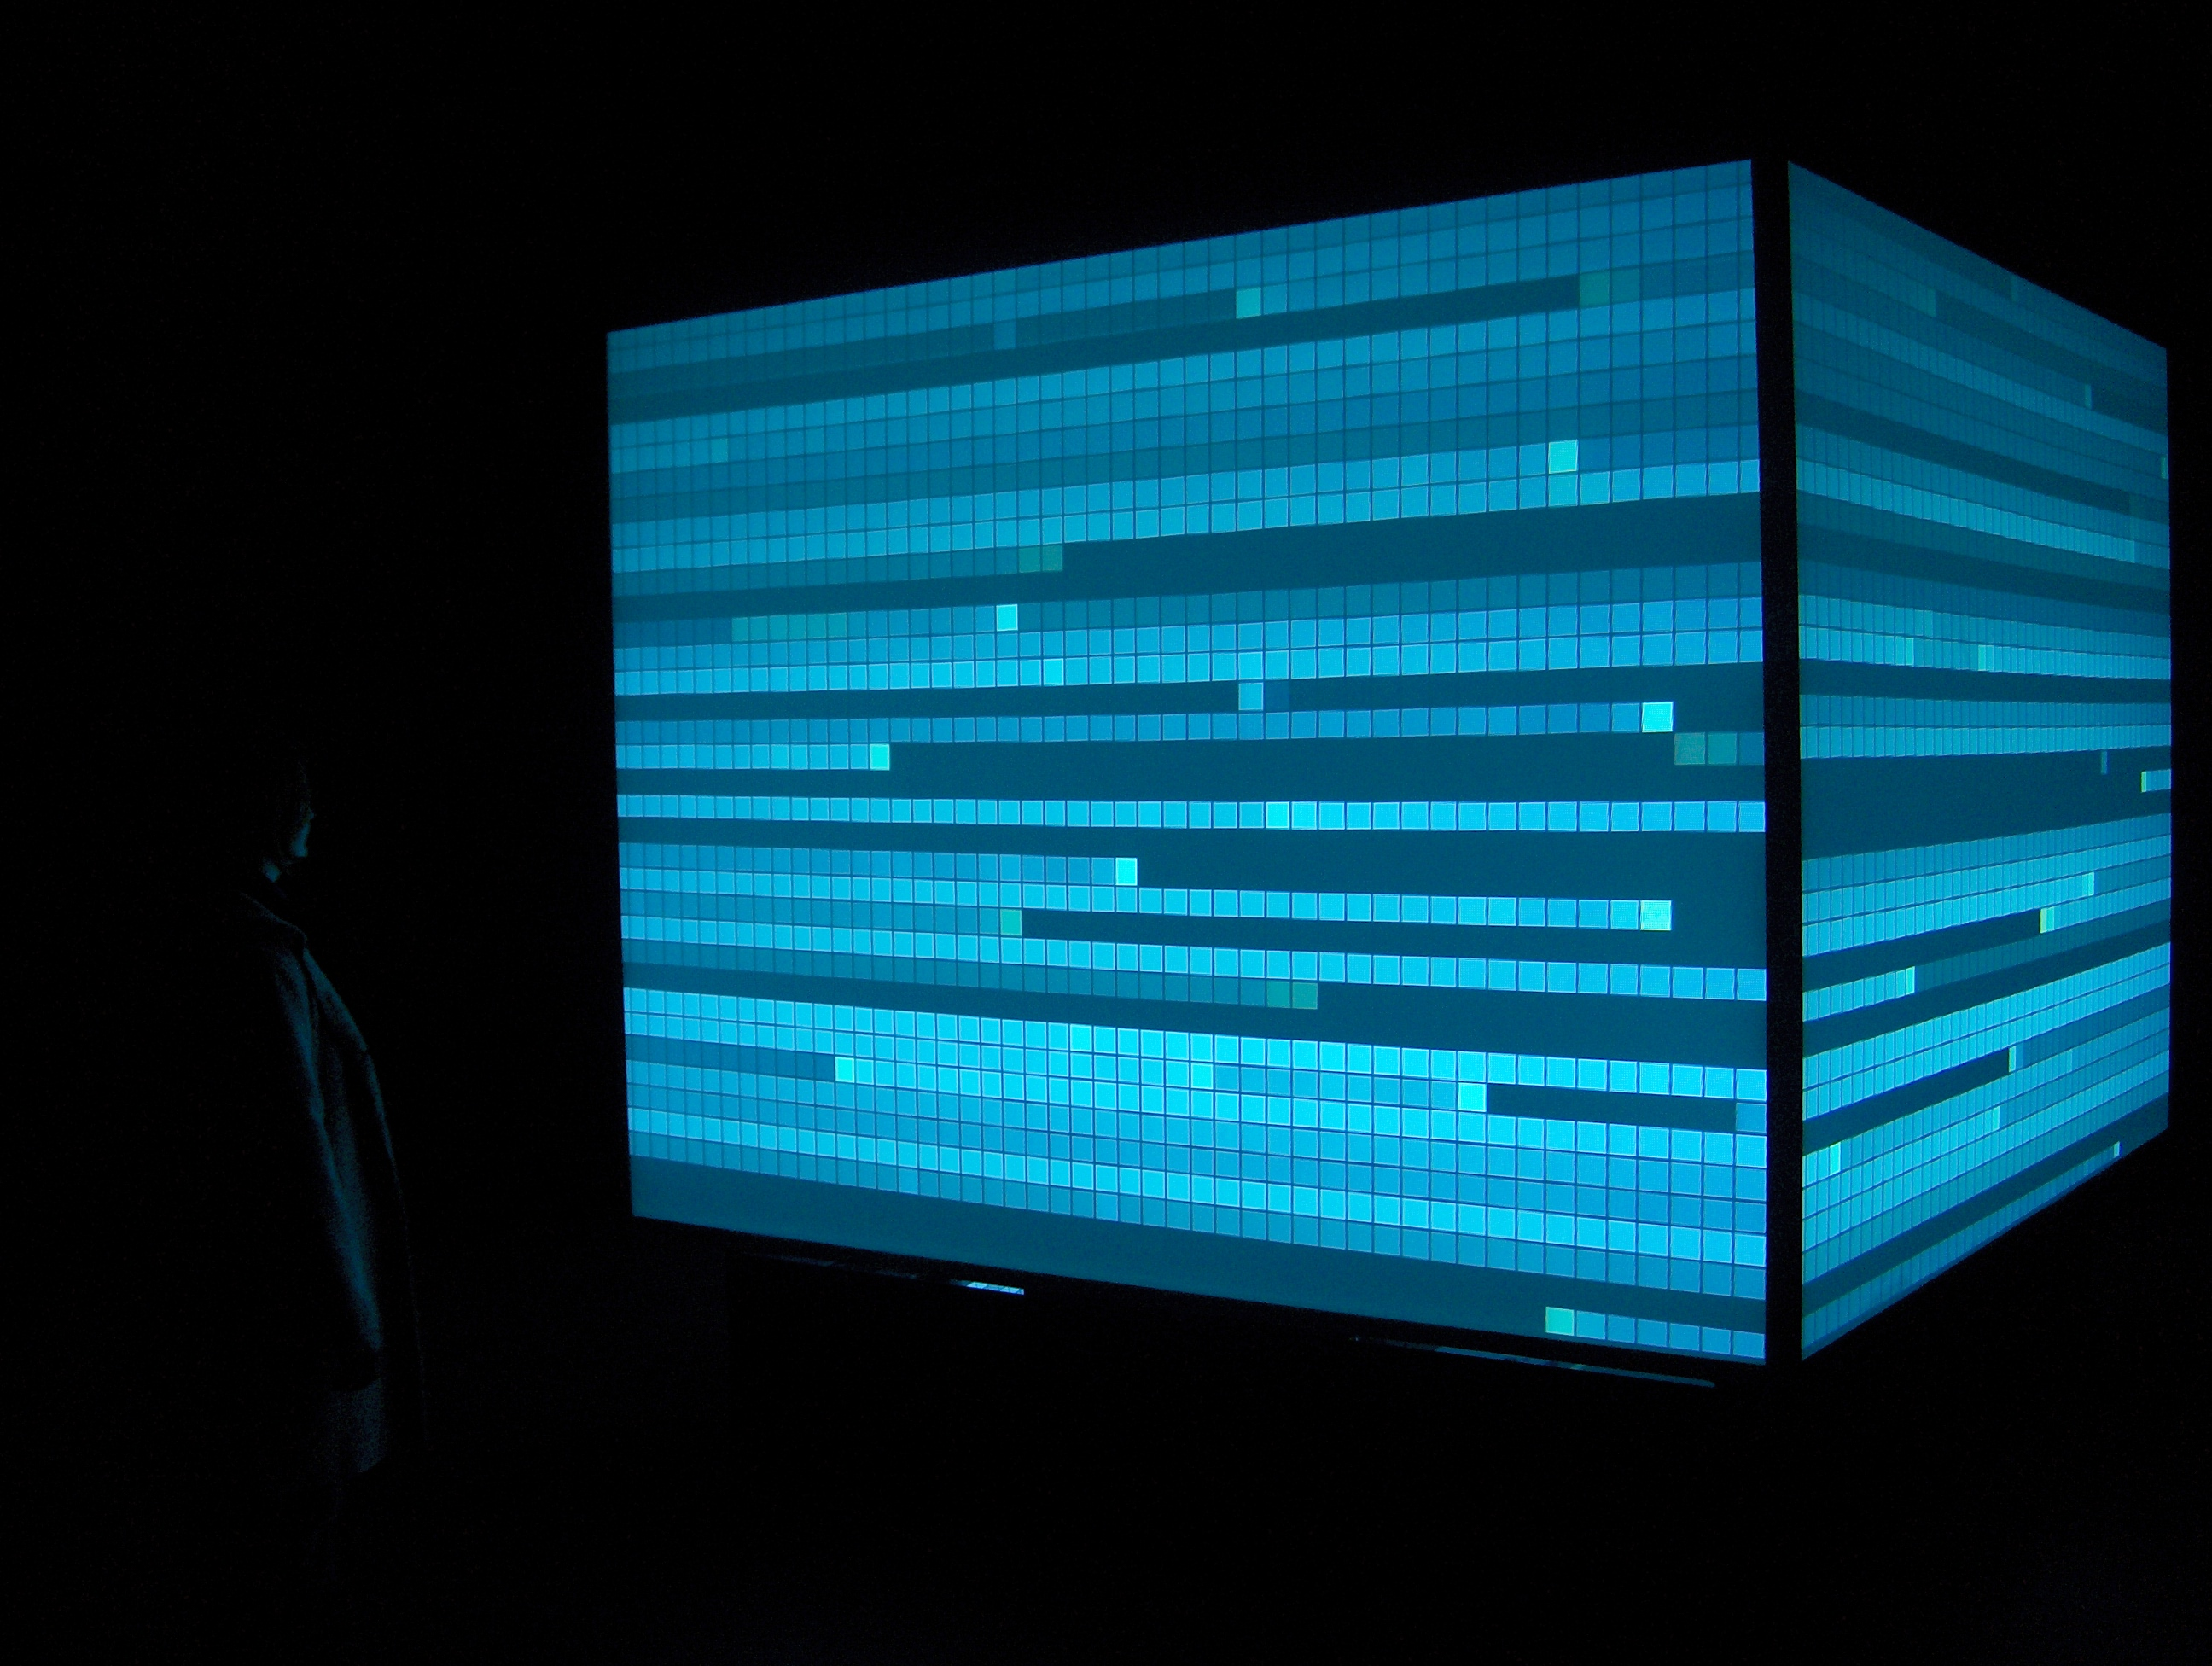
\includegraphics[height=4cm]{images/sonik6.jpg}
	\end{figure}
 \end{column}

 \begin{column}{0.4\textwidth}
	\begin{figure}
	\centering
	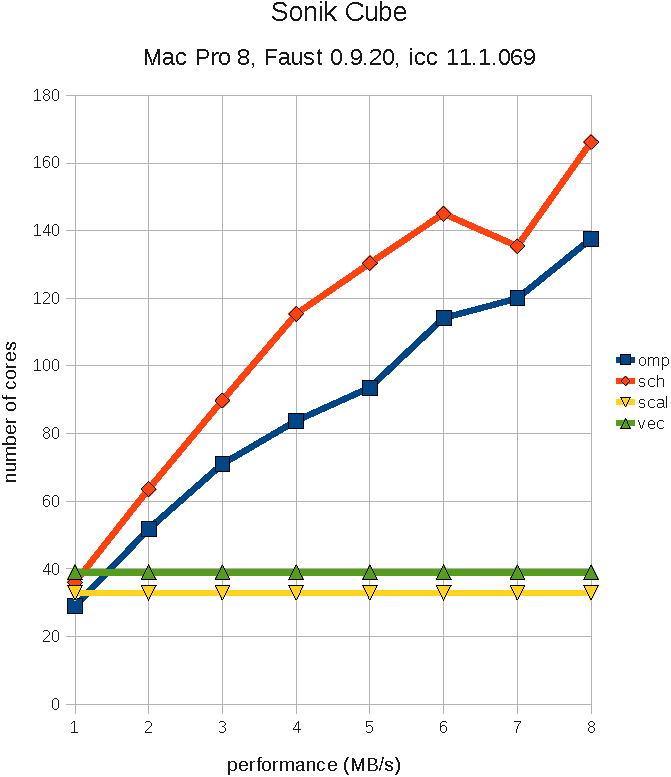
\includegraphics[height=5cm]{images/ethersonik-bench}
	\end{figure}
 \end{column}

\end{columns}

\end{frame}
